\documentclass[addpoints,a4paper]{exam}

\usepackage{amsmath, amsfonts, amssymb, amsthm}
\usepackage{graphicx}
\usepackage{hyperref}
\usepackage{tabularx}
\usepackage{pythonhighlight}

\printanswers

\begin{document}
\begin{flushleft}
  { \large \textsf{\textbf{Spring 2022, CS 412: Algorithms: Design and Analysis,  Quiz 6 -- L3}}}\vspace{.5em}

  Friday, 29 April, 2022. Total Marks: \numpoints, Duration: 20 minutes.
\end{flushleft}

\noindent{\bf Instructions:}\\
--- You have to implement the function, \pyth{solve()}, included in the accompanying file, \texttt{tower.py}.\\
--- Test your implementation by running \pyth{pytest}.\\
--- Do not include any external packages. \href{https://docs.python.org/3.8/py-modindex.html}{Built-in packages} may be used.\\
--- Do not use any python features more recent than python 3.8.\\
--- Once you are satisfied with your code, push it to your repository where it will be subjected to the same \pyth{pytest} tests. Failure to comply with the above instructions may cause your tests to fail.\\
--- There are 45 tests. Your score is the number of tests that successfully pass \textit{on GitHub} provided they are not hard-coded.\\
--- You may use online resources, e.g. to look up language features, provided you do not look up the solution to the problem.\\

\centerline{\rule{.7\textwidth}{1pt}}

\begin{questions}
\question[45] The problem is described below with one exception. The description requires to read the input and print the output. Instead, your function, \pyth{solve()}, will take the input as argument and return the desired output as a \pyth{list} of integers.
  
\noindent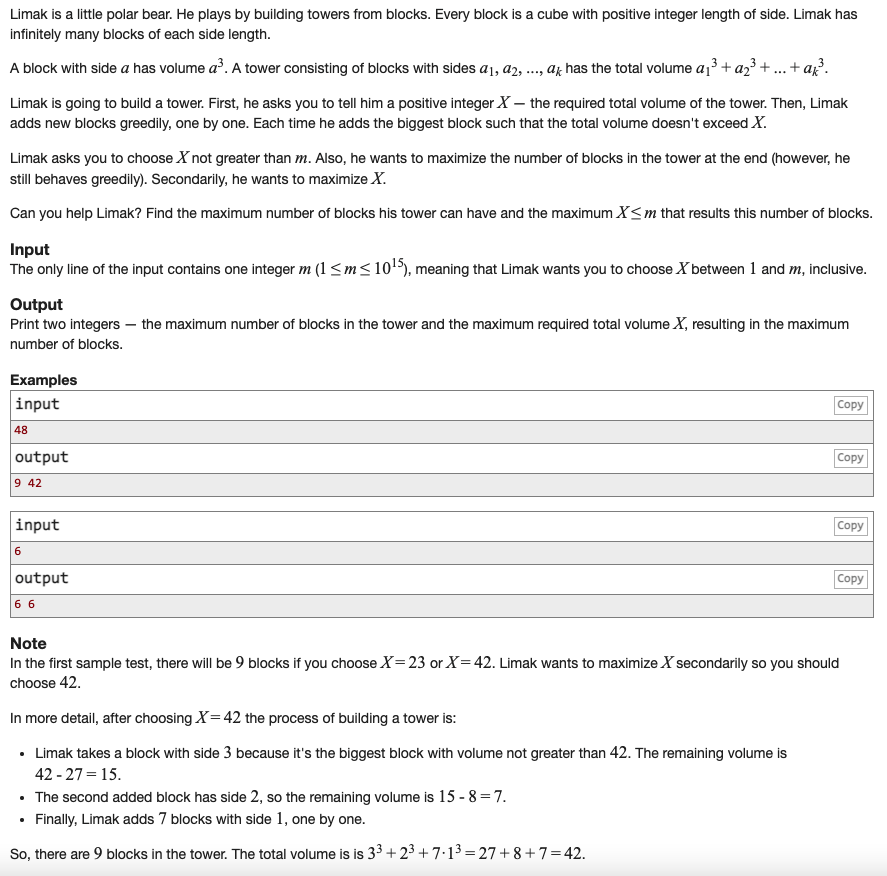
\includegraphics[width=\textwidth]{problem}
\centerline{\rule{.3\textwidth}{1pt}viel Gl\"uck\rule{.3\textwidth}{1pt}}
\end{questions}
  

\end{document}

%%% Local Variables:
%%% mode: latex
%%% TeX-master: t
%%% End:
